\section{تصویر برداری موازی}

در این قسمت برای سرعت بخشیدن به فرایند تصویربرداری \mri روش هایی معرفی می‌شود که به تصویر برداری موازی 
\LTRfootnote{Parallel Imaging}
موسوم هستند.
در تصویربرداری \mri دادگان مستقیما از تصویر برداشته نمی‌شوند بلکه از فضای فوریه ‌ی تصویر موسوم به \kspace اخذ می‌شوند. (شکل \ref{fig:kspace-fov-res})






\begin{figure}[t!]
	\centering
	\begin{RTLcopyrightBox}{\linewidth}{\doiSource{10.1002/jmri.23639}}
		\subfigure[میدان دید کامل و رزولوشن کامل]{
			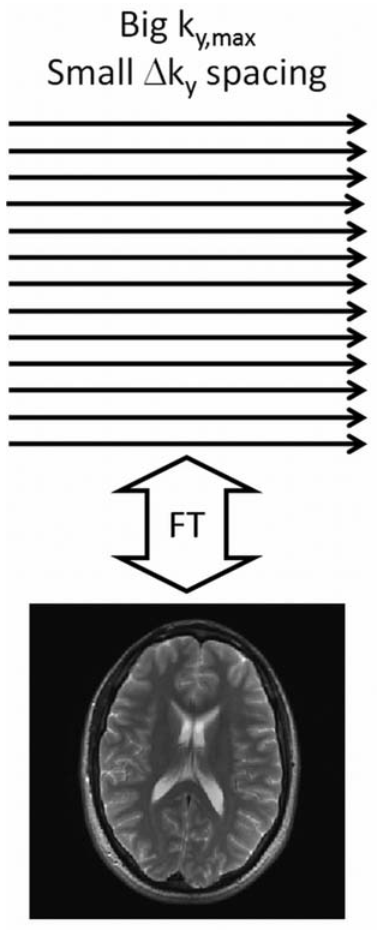
\includegraphics[width=0.3\linewidth]{chapters/chapter-3/figs/kspace-full-fov-full-res}
			\label{subfig:kspace-full-fov-full-res}}
		\hfill
		\subfigure[میدان دید کامل و رزولوشن کمتر]{
			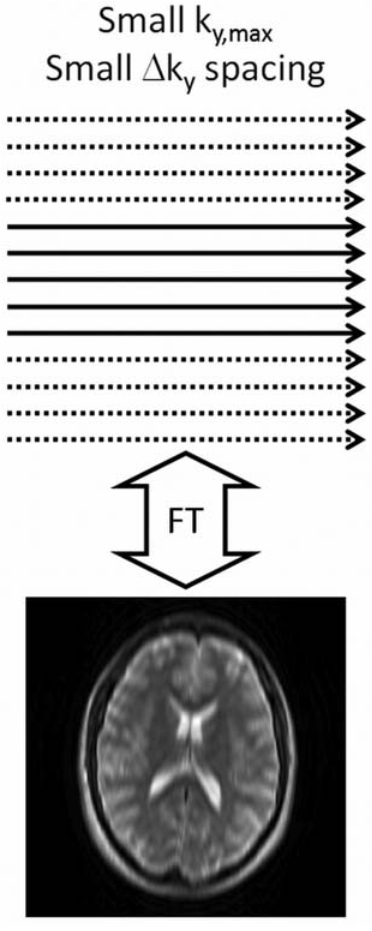
\includegraphics[width=0.3\linewidth]{chapters/chapter-3/figs/kspace-full-fov-lower-res}
			\label{subfig:kspace-full-fov-lower-res}}
		\hfill
		\subfigure[میدان دید کمتر و رزولوشن کامل]{
			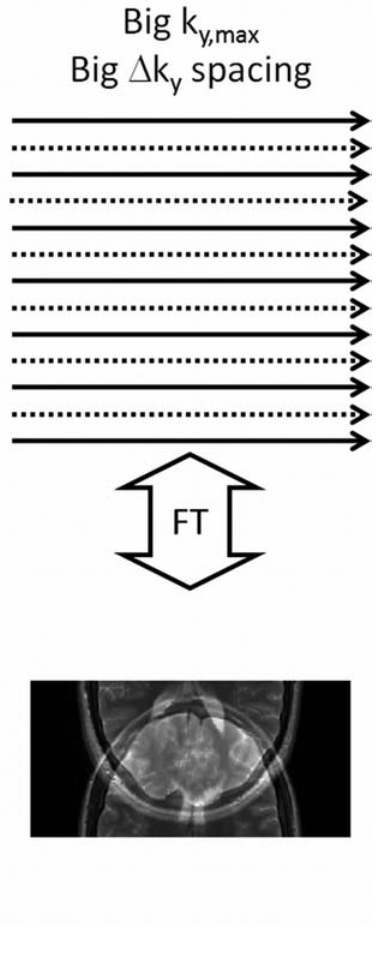
\includegraphics[width=0.3\linewidth]{chapters/chapter-3/figs/kspace-smaller-fov-full-res}
			\label{subfig:kspace-smaller-fov-full-res}}
		\hfill
	\end{RTLcopyrightBox}
	\removevspace
	\caption{}
	\label{fig:kspace-fov-res}
\end{figure}







سیگنال های بدست آمده عموما در جهت $k_x$ به صورت فرکانسی کد می‌شوند و در جهت $k_y$ به صورت خطوطی از کد کردن فاز می‌باشند. همچنین اگر تصویر برداری سه بعدی مدنظر باشد یک کد کردن دوم فاز نیز در جهت $k_z$ صورت می‌گیرد. زمان کل اخذ داده
\LTRfootnote{Total acqusition time}($T_A$)
برای یک اسکن دو بعدی به صورت زیر می‌باشد.

\removevspace
\begin{equation}
T_A = T_R \times N_{PE}
\end{equation}

که $T_R$ زمان تکرار
\LTRfootnote{Repetition time}
یا زمانی که نیاز است تا یک خط از \kspace در طول $k_x$ دریافت شود می‌باشد. همچنین $N_{\mathrm{PE}}$ نیز تعداد خطوط کد کردن فاز در جهت $k_y$ می‌باشد. در یک تصویر برداری سه بعدی، تعداد کد کردن پارتیشن ها
\LTRfootnote{Partition encoding}
($N_{\mathrm{PART}}$)
نیز باید به حاصل ضرب اضافه کرد.

$T_R$
کمک می‌کند که کنتراست تصویر را تنظیم کنیم و $N_{\mathrm{PE}}$
روزولوشن تصویر در جهت کدکردن فاز را تعیین می‌کند.

برای کاهش زمان استخراج داده، یا باید داده های \kspace سریع‌تر استخراج شود(که به معنی کاهش زمان $T_R$
است) و یا تعداد داده کمتری استخراج شود (که به معنای کاهش $N_\mathrm{PE}$ می‌باشد).


سرعت جمع آوری داده های \kspace، کنتراست مطلوب تصویر را تنظیم می‌کند. برای بعضی از انواع اسکن مانند اسپین اکو
\LTRfootnote{Spin Echo}
، $T_R$ باید به اندازه ای باشد تا کنتراست مطلوب تصویر تولید شود. در باقی انواع اسکن مانند 
گرادیان
\LTRfootnote{Spoiled Gradient Echo}
یا سری‌های تقدیمی آزاد حالت ماندگار متعادل
\LTRfootnote{Balanced Steady-State Free-Precession Sequences}
، کاهش زمان $T_R$ با حفظ کنتراست تصویر ممکن است.

اما یک محدودیت فیزیکی نیز وجود دارد. قطع و وصل کردن سریع گرادیان با میدان قوی می‌تواند یک جریان الکتریکی در بدن بیمار القا کند که آن نیز می‌تواند بالقوه باعث ایجاد تحریکات عصبی حاشیه‌ای
\LTRfootnote{Peripheral Nerve Stimulation}
 شود\cite{ParallelMRImaging2012}.

دیدگاه دیگر برای کاهش زمان $T_A$، کاهش تعداد داده های جمع آوری شده می‌باشد. یک راه برای این کاهش، کاهش ساده‌ی $k_{y, \max}$
می‌باشد در حالی که فاصله‌ی $\Delta k_y$ حفظ شده است (شکل \ref{subfig:kspace-full-fov-lower-res}).
از آن جا که طبق رابطه \ref{eq:fov-res-kspace}
رزولوشن در جهت $y$ با معکوس $k_{y,\max}$ متناسب است، این کار باعث کاهش رزولوشن تصویر و مات شدن آن می‌شود.
اگر رزولوشن تصویر بخاطر مسایل کلینیکالی بخواهد ثابت بماند، یک راه آن است که مانند شکل \ref{subfig:kspace-smaller-fov-full-res} برخی از خطوط کدکردن فاز حذف شوند. با این کار $\Delta k_y$ زیاد می‌شود و مطابق رابطه‌ی \ref{eq:fov-res-kspace} باعث کاهش در میدان دید تصویر می‌شود که درصورتی که ابعاد شئ از ابعاد میدان دید بزرگتر باشد، می‌تواند باعث ایجاد اختلاط مکانی
\LTRfootnote{Spatial Aliasing}
می‌شود. در حقیقت \lr{FOV} (که توسط فاصله‌ی خطوط کد کردن فاز تعیین می‌شود)، باید حداقل به بزرگی ابعاد شئ مورد تصویر برداری باشد. این الزام بر روی \lr{FOV} و محدوده‌ی نمونه برداری \kspace به عنوان نرخ نایکویست
\LTRfootnote{Nyquist criterion}
شناخته می‌شود. اگر نرخ نایکوییست در هردو جهت $k_x$ و  $k_y$ رعایت شود، تصویر می‌تواند مانند شکل \ref{subfig:kspace-full-fov-full-res}
بدون اختلاط مکانی بازسازی شود.



\subsection{روش های تصویربرداری موازی}

هنگامی که سرعت بخشیدن به جمع آوری داده های \mri با جمع آوری تعداد کمتری خطوط کدکردن فاز ممکن است که قبل از استفاده تصاویر در کاربرد های کلینیکی، اختلاط مکانی آن ها حذف شود. روش های تصویربرداری موازی در راستای حل کردن این مشکل، ایجاد شده اند. همه روش های تصویربرداری موازی سه مشخصه‌ی زیر را مشترک دارند:


\begin{enumerate}
	\item
	داده های \kspace
\end{enumerate}


\begin{figure}[t!]
	\centering
	\subfigure[]{
		\copyrightbox[b]{
			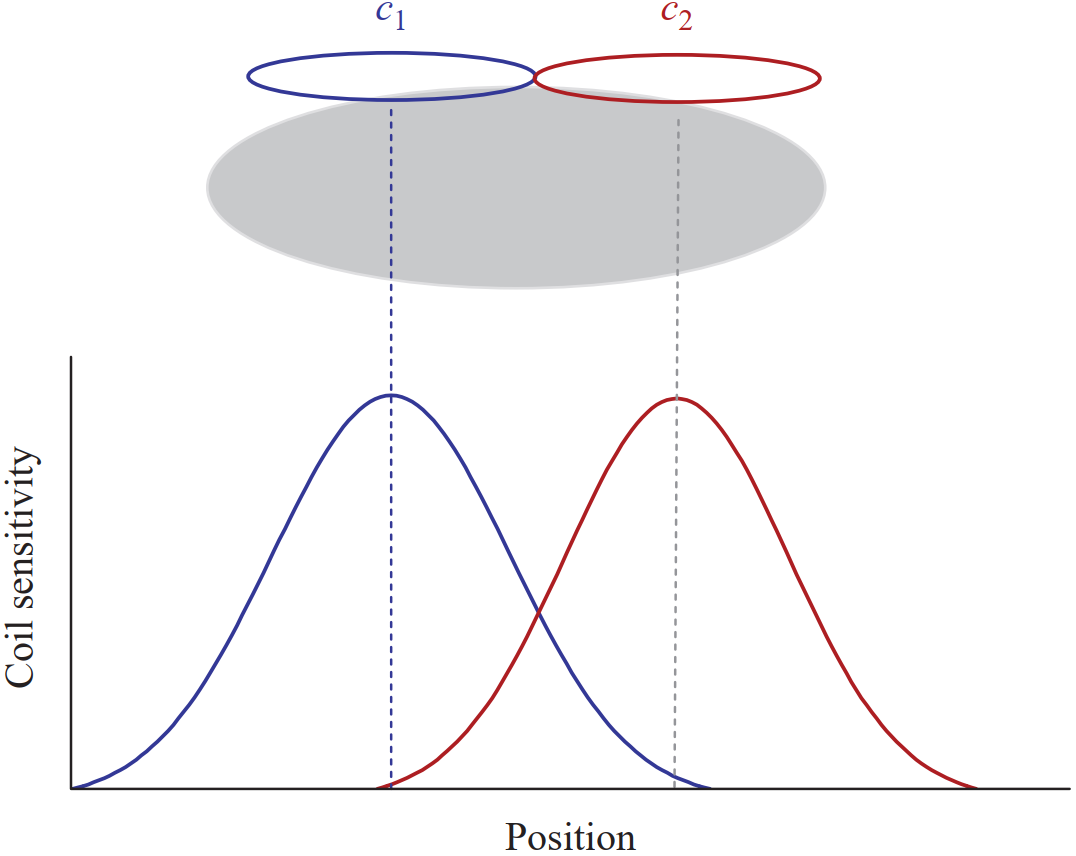
\includegraphics[width=0.45\linewidth]{chapters/chapter-3/figs/coil-sensivity-2}
		}{\doiSource{10.1017/CBO9780511545405}}}
	\hfill
	\subfigure[]{
		\copyrightbox[b]{
			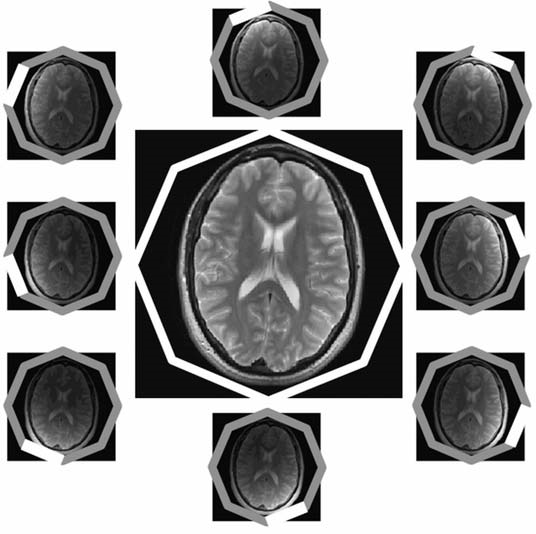
\includegraphics[width=0.36\linewidth]{chapters/chapter-3/figs/coil-sensivity-8}
		}{\doiSource{10.1002/jmri.23639}}}
	\removevspace[1]
	\caption{}
\end{figure}






\begin{figure}[t!]
	\centering
	\copyrightbox[b]{
		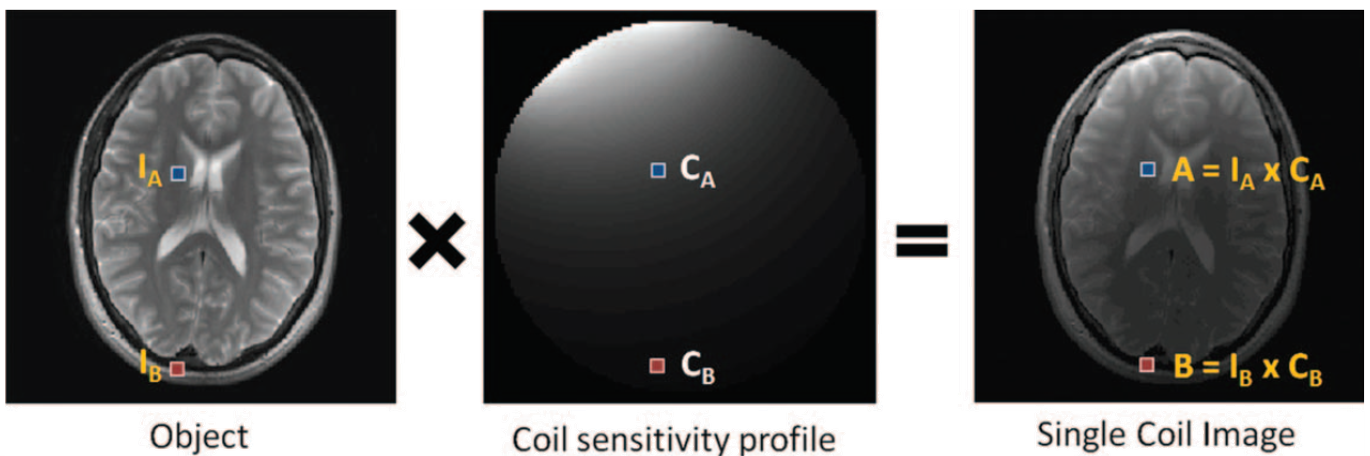
\includegraphics[width=0.9\linewidth]{chapters/chapter-3/figs/coil-sensivity-product}
	}{\doiSource{10.1002/jmri.23639}}
	\removevspace[1]
	\caption{}
\end{figure}

















